% Notes on TCDB classifier system
% june 2015
\documentclass[english]{article}
%\usepackage[T1]{fontenc}
%\usepackage[latin9]{inputenc}
%\usepackage[margin=10pt,font=small,labelfont=bf,labelsep=endash]{caption}

\usepackage{amssymb}
\usepackage{amsmath}
\usepackage{amsfonts}
%\usepackage{stmaryrd}
\usepackage[dvips]{graphicx}
\usepackage{fancybox}
\usepackage{textcomp}
\usepackage{enumerate}
%\usepackage{hyperref}

\newcommand{\inda}{\phantom{1}\hspace{3mm}}
\newcommand{\indb}{\phantom{1}\hspace{8.5mm}}
\newcommand{\indc}{\phantom{1}\hspace{12mm}}
\newcommand{\indd}{\phantom{1}\hspace{16mm}}
\newcommand{\inde}{\phantom{1}\hspace{20mm}}
\newcommand{\indf}{\phantom{1}\hspace{24mm}}
\newcommand{\indg}{\phantom{1}\hspace{28mm}}


\newcommand{\bk}{\boldsymbol{k}}
\newcommand{\bx}{\boldsymbol{x}}
\newcommand{\bp}{\boldsymbol{p}}
\newcommand{\bs}{\boldsymbol{s}}
\newcommand{\bt}{\boldsymbol{t}}
\newcommand{\bq}{\boldsymbol{q}}
\newcommand{\bw}{\boldsymbol{w}}
\newcommand{\bW}{\boldsymbol{W}}
\newcommand{\bL}{\boldsymbol{L}}
\newcommand{\bD}{\boldsymbol{D}}
\newcommand{\bI}{\boldsymbol{I}}
\newcommand{\bK}{\boldsymbol{K}}
\newcommand{\bQ}{\boldsymbol{Q}}
\newcommand{\bE}{\boldsymbol{E}}
\newcommand{\bM}{\boldsymbol{M}}
\newcommand{\F}{\boldsymbol{F}}
\newcommand \ignore[1] {}

\newtheorem{theorem}{Fact}


\begin{document}



\title{Notes on the development of an automated predictor for the Transporter Classification Data-Base (TCDB)}

\author{}
\maketitle

\tableofcontents





%%%%%%%%%%%%%%%%%%%%%%%%%%%%%%%%%%%%%%%%%%%%%%%%%%%%
\section{Classification criteria underlying the TCDB}
\label{}
The TCDB website details a comprehensive classification system for membrane transport proteins known as the Transport Classification (TC) system. The TC system is analogous to the Enzyme Commission (EC) system for classification of enzymes, except that it incorporates both functional and phylogenetic information~\cite{Saier06,Saier14}. 
Basically the taxonomy is based on the mode of action of the transport activity and the energy coupling mechanism used for the transport.
Phylogenetic grouping reflects structure, function, mechanism, and often substrate specificity and therefore provides a reliable secondary basis for classification. Finally substrate specificity and polarity of transport provide a tertiary basis for classification.

Schematically, the basic criteria of classification proposed in the TCDB are the following~\cite{Saier00}:
\begin{enumerate}[i.]
\item transport mode
\item energy coupling mechanism
\item phylogenetic grouping
\item substrates transported
\end{enumerate}


These criteria of classification are reflected in the 5-tier taxonomy, coded by 5  point separated digits V.W.X.Y.Z:
\begin{enumerate}
\item W (a number): the first level of the hierarchy, i.e. the class of the transport protein. It corresponds to the most general classes of the taxonomy.
\item V (a letter): the second level of the hierarchy, i.e. the subclass of the transport protein. 
\item X (a number): the third level of the hierarchy, i.e. the family (sometimes the superfamily) of the transport protein. 
\item Y (a number): the fourth level of the hierarchy, i.e. the subfamily  
\item Z (a number): the fifth level of the hierarchy is mostly related to the substrate(s) on which the transport proteins acts. 
\end{enumerate}



%%%%%%%%%%%%%%%%%%%%%%%%%%%%%%%%%%%%%%%%%%%%%%%%%%%%
\subsection{Structure of TCDB}
\label{}
TCDB is a 5-tier taxonomy of transport proteins structured according to a tree.
We have the following per-level distribution of the $12587$ classes (from top to bottom):
\begin{enumerate}
\item level 1: 7  
\item level 2: 30
\item level 3: 867
\item level 4: 2235
\item level 5: 9448 
\end{enumerate}




%%%%%%%%%%%%%%%%%%%%%%%%%%%%%%%%%%%%%%%%%%%
\begin{table}[!h]
\caption {Distribution of the cardinality of the classes.
The number of annotated proteins is $12508$ belonging to at least $2574$ different species.}
\label{tab:datasources}
\vskip 0.05in
\centering
%\begin{sc}
\begin{tabular}{| r | r |}
\hline
 \textbf{Number of annotations} 		&		\textbf{Number of classes}	 \\ 
 \hline
 1    &   9173 \\ \hline
 $> 1$   &   3414 \\ \hline
 $> 5 $     &   1245 \\ \hline
 $> 10$      &   597    \\ \hline
$ > 20 $        &   232   \\ \hline
 $> 50$        &   67   \\ \hline
 $> 100$ & 37  \\ \hline
 $> 200$  & 24  \\ \hline
 $> 500$ & 12  \\ \hline
 $> 1000$          &  10   \\
\hline
\end{tabular}
%\end{sc}
\normalsize
\end{table}
%%%%%%%%%%%%%%%%%%%%%%%%%%%%%%%%%%%%%%%%%%%


%%%%%%%%%%%%%%%%%%%%%%%%%%%%%%%%%%%%%%%%%%%%
\begin{table}[h!]
\caption {Per-level distribution of the per-class TCDB annotations}
\label{tab:distr-per-level}
%\vskip 0.15in 
\begin{center}
\begin{normalsize}
%\begin{sc}
\begin{tabular}{|c|r|r|r|r|r|r|}
\hline
%\abovespace\belowspace
    	&  \textsc{Min}  & \textsc{1st Qu.}  & \textsc{Median} & \textsc{Mean} & \textsc{3rd Qu.}  &  \textsc{Max}\\  \hline
Level 1  &  131  &   318 &   1391 &   1788  &  3408  &  3542     \\ \hline 	
Level 2  &  1 &  19  & 56 & 417&  426& 3416     \\ \hline
Level 3  &  1 &   2 &   6 &  14.4 &  12& 1661    \\ \hline
Level 4  &  1 &  1&   3 &  5.6  & 6& 196    \\ \hline
Level 5  &  1 &  1  & 1 &  1.3 &  1 & 45    \\ \hline
\hline
\end{tabular}
\end{normalsize}
\end{center}
%\vskip -0.1in
\end{table}
%%%%%%%%%%%%%%%%%%%%%%%%%%%%%%%%%%%%%%%%%%%%%%%%%%%%%%%%%%%%%%%%%%


	



%%%%%%%%%%%%%%%%%%%%%%%%%%%%%%%%%%%%%%%%%%%%%%%%%%%%%%%%%%%%%%%%
\begin{figure}[!h]

\includegraphics[width=15cm]{fig/TCDB2level.ps} 
\caption{The first two levels of the TDCB taxonomy. 0 is a dummy added node to obtain a tree instead of a forest.}
\label{fig:two-levels}
\end{figure}


%%%%%%%%%%%%%%%%%%%%%%%%%%%%%%%%%%%%%%%%%%%%%%%%%%%%%%%%%%%%%%%%
\begin{figure}[!h]

\includegraphics[width=15cm]{fig/TCDB3level.ps} 
\caption{The first three levels of the TDCB taxonomy}
\label{fig:three-levels}
\end{figure}

%%%%%%%%%%%%%%%%%%%%%%%%%%%%%%%%%%%%%%%%%%%%%%%%%%%%
\subsection{The levels of the TCDB hierarchy}
The different levels articulates the function and the phylogenetic characeristics of the transport proteins across all the living organisms.

%%%%%%%%%%%%%%%%%%%%%%%%%%%%%%%%%%%%%%%%%%%%%%%%%%%%
\subsubsection{The class level}
It represents the highest level of classification reflecting the general transport mode as well as the way in which energy is exploited to perform the transport (Tab.~\ref{tab:first-level}). Fig.~\ref{fig:card-level1} provides a summary of the cardinality of the $7$  protein transport categories defined at this level (note that classes 6 and 7 are left undefined for possible future rearrangements of the hierarchy).


%%%%%%%%%%%%%%%%%%%%%%%%%%%%%%%%%%%%%%%%%%%
\begin{table}[!h]
\caption {Characteristics of the most general classes (first level) of the hierarchy}
\label{tab:first-level}
\vskip 0.05in
\hspace{-2cm}
%\begin{sc}
\begin{tabular}{| l | l | l |}
\hline t
\textbf{Code}  & \textbf{Name of the class} 		&		\textbf{Short description}	 \\ 
 \hline
 1    & Channels/Pores  &  catalyze facilitated diffusion  \\
       &     & (by an energy-independent process) \\
   &     &   by passage through a transmembrane  \\
   &     &   aqueous pore or channel \\
   &     &   without evidence for \\
   &     &   a carrier-mediated mechanism \\ \hline
2  &  Electrochemical Potential  & utilize a carrier-mediated process \\
   &   driven Transporters  &  not directly linked to a form of energy \\ 
   &     &   other than chemiosmotic energy   \\ \hline
 3     & Primary Active Transporters  &  use a primary source of energy \\ 
   &     &   (chemical, electrical or solar) \\ 
   &     &   to drive active transport of a \\ 
   &     &    solute against a concentration gradient  \\ \hline
 4      & Group Translocators  &  involves a combined chemical and vectorial \\
   &     &   reaction where the transported substrate\\
      &     &   is modified during the transport process  \\ \hline
5  & Transmembrane Electron Carriers  &   systems that catalyze electron flow across\\
       &     &    a biological membrane, from donors to acceptors    \\ \hline
 8   & Accessory Factors Involved in Transport  &   proteins that in some way facilitate transport  \\
       &     &  but do not participate directly in transport  \\ \hline
 9 &Incompletely Characterized &  Transporters of unknown classification\\
  &   Transport Systems  & \\ \hline
\hline
\end{tabular}
%\end{sc}
\normalsize
\end{table}
%%%%%%%%%%%%%%%%%%%%%%%%%%%%%%%%%%%%%%%%%%%


  
 
 

%%%%%%%%%%%%%%%%%%%%%%%%%%%%%%%%%%%%%%%%%%%%%%%%%%%%%%%%%%%%%%%%
\begin{figure}[!h]

\includegraphics[width=12cm]{fig/CardLevel1.ps} 
\caption{Cardinality of the most general classes (Level 1)}
\label{fig:card-level1}
\end{figure}


%%%%%%%%%%%%%%%%%%%%%%%%%%%%%%%%%%%%%%%%%%%%%%%%%%%%
\subsubsection{The subclass level}
This level provides a further specification of the main mode of action and energy mechanism underlying the transporter.
For instance in the case of primary active transporters(class 3)  refers to the energy source used to drive transport, i.e. chemical (3.A P-P bond hydrolisis, 3.B decarboxylation-driven, 3.C methyltransfer-drive), electrical (3.D oxidoreduction-driven), and solar (3.E light absorption-driven), or in the case of Class 1 (channels and pores) fundamental structural differences lead to different subclasses such as proteins characterized by $\alpha$-elical portions, ubiquitously found i all organisms(1.A $\alpha$- Type channels) and proteins whose transmembrane potions are characterized by $\beta$-strands found usually in Bacteria (1.B $beta$-Barrel porins).


%%%%%%%%%%%%%%%%%%%%%%%%%%%%%%%%%%%%%%%%%%%%%%%%%%%%
\subsubsection{The family level}
A phylogenetic family of transporters includes members that function by a single transport mode and energy coupling mechanism, although a variety of substrates may be transported~\cite{Saier00}. 
It should be noted that this level corresponds to phylogenetically related proteins, whose evolution reflects common modes of transports and common ways to exploit energy to realize transport functions. Families are based on (limited) sequence or motif similarity, similar protein size, topology and structure (when available).

Some of these families are actually large superfamilies with more than a thousand currently sequenced members (e.g., the voltage-gated ion channel (VIC) family -- TC 1.A.1) Others are very
small families with only one or a few currently sequenced members.

%%%%%%%%%%%%%%%%%%%%%%%%%%%%%%%%%%%%%%%%%%%%%%%%%%%%
\subsubsection{The subfamily level}
This level corresponds to a further phylogenetic separation inside families that may correspond also to slightly different functions or actions on different substrates. In some cases they could be also families, when the previous level corresponds to a superfamily. We could try to predict till to this level.

%%%%%%%%%%%%%%%%%%%%%%%%%%%%%%%%%%%%%%%%%%%%%%%%%%%%
\subsubsection{The most specific level}
This level delineates the substrate or range of substrates transported as well as the polarity of transport. 
Any two proteins  in the same subfamily that transport the same substrate(s) using the same
mechanism are given the same TC number, regardless of whether they are orthologs (i.e., arose in distinct organisms by
speciation) or paralogs (i.e., arose within a single organism by gene duplication).
The predictions at this level seem quite difficult since we have usually only 1 protein annotated at this level, and when we have more proteins annotated for a class as this level, this means that they belong to the same transport system or a complex exploiting a specific transport function with a specific mode of action and energy coupling and on specific substrates.


%%%%%%%%%%%%%%%%%%%%%%%%%%%%%%%%%%%%%%%%%%%%%%%%%%%%
\subsection{Remarks on the TCDB annotations}

\subsubsection{Meaning of the multiple annotations for the most specific classes.}
At level 5 the class having 45 annotations is  3.D.1.6.1: The animal H+-translocating NADH dehydrogenase (NDH) complex (Table~\ref{tab:distr-per-level}).
This is  a complex of the mitochondrial inner  membrane involved in the respiratory chain. This complex is composed by 45 subunits and the 45 annotations correspond exactly to the 45 protein subunits.

This is true also for 3.D.1.6.2: The fungal H+ translocating NADH dehydrogenase (NDH) complex having 31 subunits and 31 annotations, for 3.D.1.6.2: The green algal H+ translocating NADH dehydrogenase (NDH) complex having 33 subunits and 33 annotations, and for 1.I.1.1.1: The Nuclear Pore Complex (NPC) in Yeast, a transport system with 35 components corresponding to 35 different proteins.

More in general, of the 9845 classes at the fifth level, 985 have more than 1 annotation. I checked by sampling 3.A.1.135.5: The heterodimeric ABC transporter that has 2 annotations corresponding to the 2 components systems (Thermatoga maritima), belonging to the  the ATP-binding Cassette (ABC) Superfamily. The 1.F.1.1.1 is a 10 component system: The Synaptosomal Vesicle Fusion Pore (SVF-Pore) having just 10 annotations. 

 Hence the classes at the fifth level having more than 1 annotation are likely those composed by different subunits/components included in the same transport system. This could be checked more in detail but I guess that this is the situation

\subsubsection{Proteins annotated to more than 1 leaf of the TCDB}
 Of the  12508 annotated proteins, only  28 have more than 5 annotations (corresponding to an unique path from the root to a leaf of the TCDB tree).
Most of them differs only at the fifth level (e.g. D4ZJA6 	Sodium-type flagellar protein MotY and  Q8EAG6 	Sodium-type flagellar protein MotX are both part of the complex
1.A.30.1.5: The H+-driven flagellar motor complexT and 1.A.30.1.5: The Na+-driven flagellar motor complex and for these reason they have a double annotation).
In other case the annotation can be different also at subfamily level (e.g.  Q03PY- Energy-coupling factor transporter ATP-binding protein EcfA1) annotated to both 3.A.1.28.2 and  3.A.1.26.9 since these different Folate-tranporters use the same energy coupling factor), or also at class level (e.g. O24303 annotated to  1.A.18.1.1 Protein import-related anion-selective channel but also as component of the complex  3.A.9.1.1 Chloroplast envelope protein translocase (CEPT)).

In any case considering that we have only 28 proteins annotated to 2 different leaves (mostly strictly related) we could consider predictions of annotations along single paths of the TCDB tree.





%%%%%%%%%%%%%%%%%%%%%%%%%%%%%%%%%%%%%%%%%%%%%%%%%%%%%%%%%%%%%%%%%%%%%%%%%%%%%%%%%%%%%%%%%%%%%%%%%%%%%%%%
\section{The data}
\label{}

An R function is available to automatically parse  any tcdb text file to automatically extract all the available fields
(SwissProt AC, TCDB code, description of the protein, gene name,  etc).
A library of R function is available for parsing the tcdb text files, construct annotations table, construct the taxonomy tree,
providing some basic statistics on the TCDB annotations.


%%%%%%%%%%%%%%%%%%%%%%%%%%%%%%%%%%%%%%%%%%%%%%%%%%%%
\subsection{Taxonomy data}
\label{}

Data of the TCDB tree are just available as graphNEL R classes or as edges in plain text files.


%%%%%%%%%%%%%%%%%%%%%%%%%%%%%%%%%%%%%%%%%%%%%%%%%%%%
\subsection{The annotation data}
\label{}

These data are just available in tabular form in both .rda R compressed files and plain text files.

%%%%%%%%%%%%%%%%%%%%%%%%%%%%%%%%%%%%%%%%%%%%%%%%%%%%
\subsection{The input feature data}
\label{}


%%%%%%%%%%%%%%%%%%%%%%%%%%%%%%%%%%%%%%%%%%%%%%%%%%%%
\subsubsection{BLAST-based data}
BLAST all vs all with TCDB proteins --> symmetric similarity matrix (data just available)

For unannotated proteins BLAST against all the TCDB proteins to obtain a feature vector.

%%%%%%%%%%%%%%%%%%%%%%%%%%%%%%%%%%%%%%%%%%%%%%%%%%%%
\subsubsection{InterPro feature data}
This data for SwissProt proteins can be extracted for UniProtKB text files.

We need to choose which features should be included.

%%%%%%%%%%%%%%%%%%%%%%%%%%%%%%%%%%%%%%%%%%%%%%%%%%%%
\subsubsection{TransMembrane Segments (TMS) data}
Available in some way from the TCDB (unfortunately there are not text files available but only data on a per-protein basis on the TCDB web-site).
TMS data could be extracted from FASTA sequences using the HMMTOP program or other similar programs. 
For a given protein we have the number of TMSs: this simple monodimensional data is useful since it can characterize classes at high level. For instance



%%%%%%%%%%%%%%%%%%%%%%%%%%%%%%%%%%%%%%%%%%%%%%%%%%%%
\subsubsection{PDB-based data}

We need to extract proper  features from the available data (Su and Jim could you provide them?).


%%%%%%%%%%%%%%%%%%%%%%%%%%%%%%%%%%%%%%%%%%%%%%%%%%%%
\subsubsection{Taxonomic data}

Considering that this taxonomy is constructed on functional, but also on phylogenetic bases, I guess that this information about the taxa will be useful. At family level some classes are characteristic or exclusive for Bacteria or Eukarya, and at subfamily or at the most specific level we are very close to the species. We should decide which level of detail could be useful for predictions at family or subfamily level. For instance in~\cite{Saier00} the categories of organisms belonging to each specific class are details at a very coarse level: Bacteria, Archaea, Eukarya, Fungi, Protozoans, Plants, Animals, etc.


%%%%%%%%%%%%%%%%%%%%%%%%%%%%%%%%%%%%%%%%%%%%%%%%%%%%
\subsubsection{Other features}
The size range (number of residues) seem to characterize different families. Hence a simple feature that could be added is for instance a binary vector with entries corresponding to the number of residues: the first entry is set to 1 if we have less than 100 residues, the second if the residue are between 100 and 200 and so on. There are problems with dimeric or multi-meric proteins (that is complexes having more than 1 subunit), that may have very large number of residues (even 6000): we could provide a further feature collection the number of subunits o the transporter  system (when o curse this data is available ...).

Another feature is the substrate on which a transporter acts. Of course this is a quite unlikely available information for uncharacterized transport proteins,  but if available could be useful. To this end we need to characterize the substrates, using, for instance, the simple taxonomy provided in Table 4 of~\cite{Saier00}.


%%%%%%%%%%%%%%%%%%%%%%%%%%%%%%%%%%%%%%%%%%%%%%%%%%%%%%%%%%%%%%%%%%%%%%%%%%%%%%%%%%%%%%%%%%%%%%%%%%%%%%%%
\section{Methods}
\label{}

%%%%%%%%%%%%%%%%%%%%%%%%%%%%%%%%%%%%%%%%%%%%%%%%%%%%
\subsection{Proposed methods}
\label{}
The taxonomy follows a tree-structure, according to the TCDB. Each annotation is articulated along a single path from the root to the leaves: in practice usually each annotated protein belongs to 5 classes, by following a unique path from the root to a specific leaf at the fifth level of the hierarchy

We could work on three (partially related) research lines:
\begin{enumerate}
\item Tree structured output methods
\item Hierarchical ensemble methods
\item Semi-supervised flat network-based methods (e.g. RANKS).

\end{enumerate}


%%%%%%%%%%%%%%%%%%%%%%%%%%%%%%%%%%%%%%%%%%%%%%%%%%%%
\subsection{Related work}
\label{}
TO DO


%%%%%%%%%%%%%%%%%%%%%%%%%%%%%%%%%%%%%%%%%%%%%%%%%%%%
\subsection{Baseline methods}
\label{}
Surely we should use BLAST methods (e.g. using the best-hit approach against the TCDB, in terms of score or p-value). Considering the way the TCDB i constructed, I guess that BLAST will be a strong baseline.
As baseline we could also use some flat machine learning-based methods. Flat machine learning-based methods could be also used as base learners with two-steps Hierarchical ensemble methods.

%%%%%%%%%%%%%%%%%%%%%%%%%%%%%%%%%%%%%%%%%%%%%%%%%%%%%%%%%%%%%%%%%%%%%%%
\bibliographystyle{plain}
\bibliography{biblioTCDB}


\end{document}
